% Created by tikzDevice version 0.12.6 on 2026-03-25 11:28:08
% !TEX encoding = UTF-8 Unicode
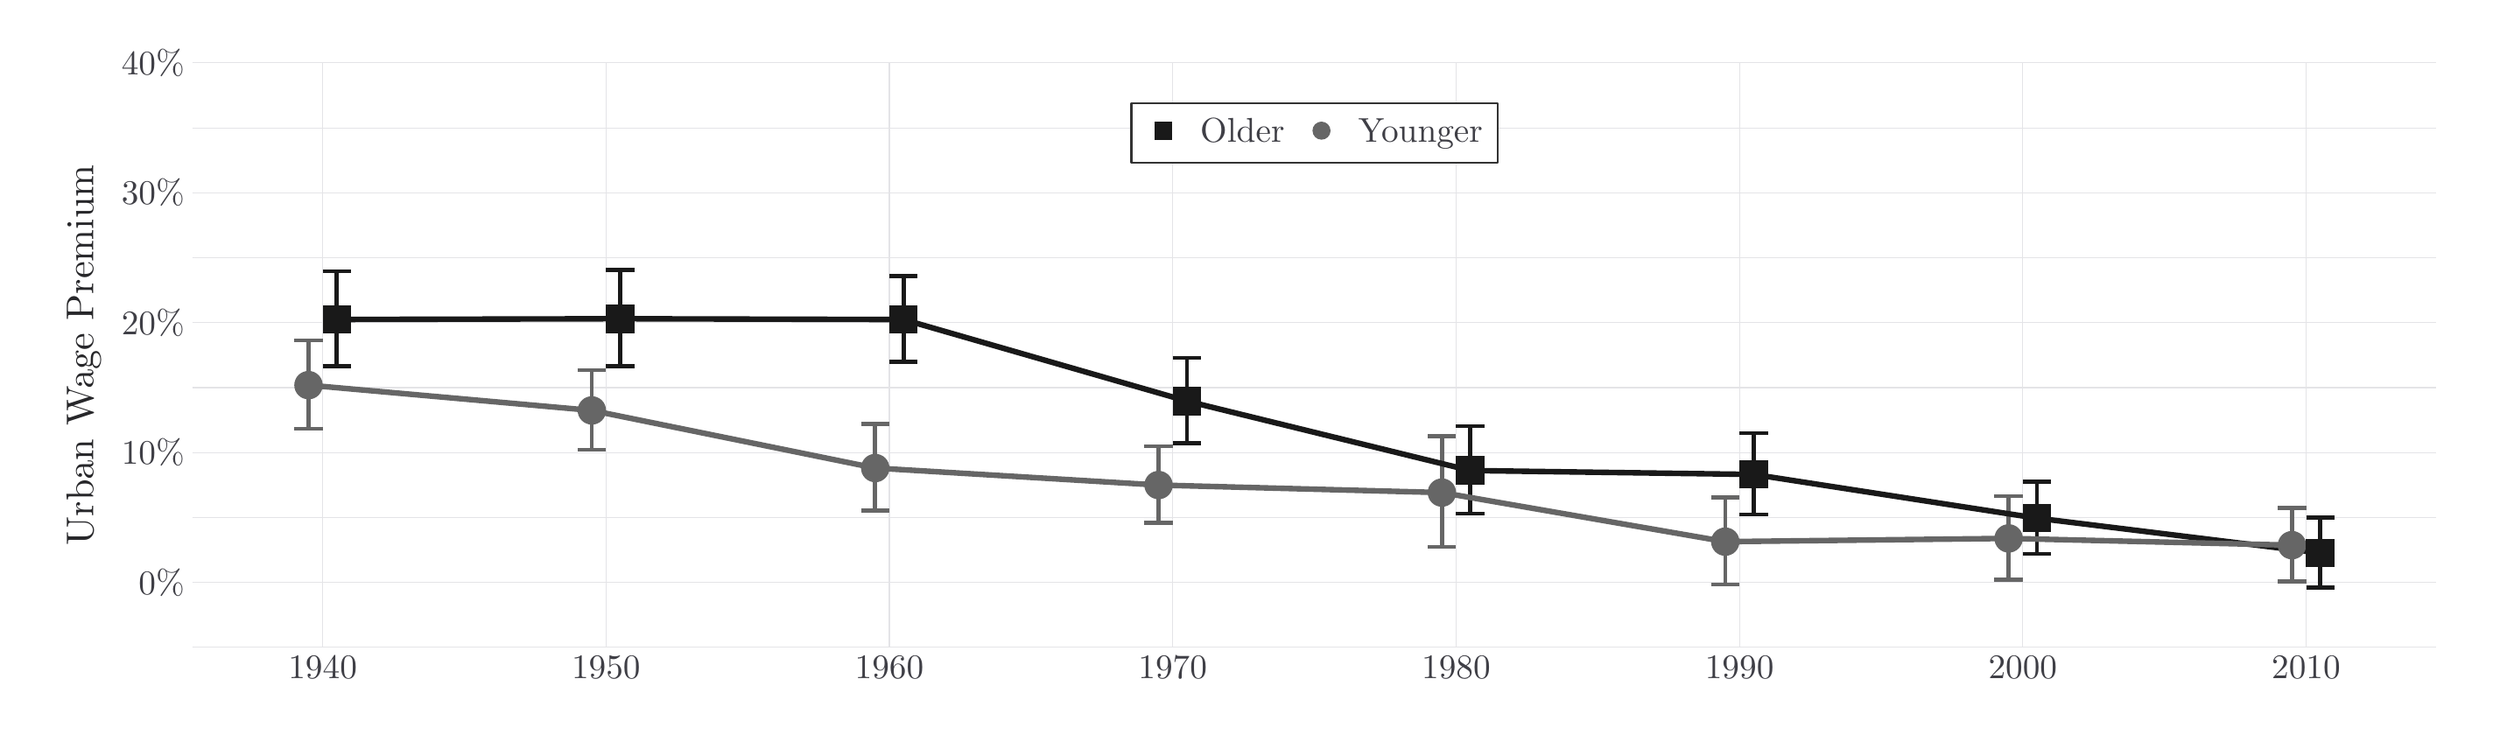
\begin{tikzpicture}[x=1pt,y=1pt]
\definecolor{fillColor}{RGB}{255,255,255}
\path[use as bounding box,fill=fillColor] (0,0) rectangle (1011.78,289.08);
\begin{scope}
\path[clip] (  0.00,  0.00) rectangle (1011.78,289.08);
\definecolor{drawColor}{RGB}{255,255,255}

\path[draw=drawColor,line width= 0.8pt,line join=round,line cap=round,fill=fillColor] (  0.00,  0.00) rectangle (1011.78,289.08);
\end{scope}
\begin{scope}
\path[clip] ( 69.39, 31.76) rectangle (995.78,273.08);
\definecolor{drawColor}{RGB}{255,255,255}
\definecolor{fillColor}{RGB}{255,255,255}

\path[draw=drawColor,line width= 0.8pt,line join=round,line cap=round,fill=fillColor] ( 69.39, 31.76) rectangle (995.78,273.08);
\definecolor{drawColor}{RGB}{228,228,231}

\path[draw=drawColor,line width= 0.4pt,line join=round] ( 69.39, 31.76) --
	(995.78, 31.76);

\path[draw=drawColor,line width= 0.4pt,line join=round] ( 69.39, 85.39) --
	(995.78, 85.39);

\path[draw=drawColor,line width= 0.4pt,line join=round] ( 69.39,139.01) --
	(995.78,139.01);

\path[draw=drawColor,line width= 0.4pt,line join=round] ( 69.39,192.64) --
	(995.78,192.64);

\path[draw=drawColor,line width= 0.4pt,line join=round] ( 69.39,246.27) --
	(995.78,246.27);

\path[draw=drawColor,line width= 0.4pt,line join=round] ( 69.39, 58.57) --
	(995.78, 58.57);

\path[draw=drawColor,line width= 0.4pt,line join=round] ( 69.39,112.20) --
	(995.78,112.20);

\path[draw=drawColor,line width= 0.4pt,line join=round] ( 69.39,165.83) --
	(995.78,165.83);

\path[draw=drawColor,line width= 0.4pt,line join=round] ( 69.39,219.45) --
	(995.78,219.45);

\path[draw=drawColor,line width= 0.4pt,line join=round] ( 69.39,273.08) --
	(995.78,273.08);

\path[draw=drawColor,line width= 0.4pt,line join=round] (123.20, 31.76) --
	(123.20,273.08);

\path[draw=drawColor,line width= 0.4pt,line join=round] (240.17, 31.76) --
	(240.17,273.08);

\path[draw=drawColor,line width= 0.4pt,line join=round] (357.13, 31.76) --
	(357.13,273.08);

\path[draw=drawColor,line width= 0.4pt,line join=round] (474.10, 31.76) --
	(474.10,273.08);

\path[draw=drawColor,line width= 0.4pt,line join=round] (591.07, 31.76) --
	(591.07,273.08);

\path[draw=drawColor,line width= 0.4pt,line join=round] (708.04, 31.76) --
	(708.04,273.08);

\path[draw=drawColor,line width= 0.4pt,line join=round] (825.01, 31.76) --
	(825.01,273.08);

\path[draw=drawColor,line width= 0.4pt,line join=round] (941.97, 31.76) --
	(941.97,273.08);
\definecolor{drawColor}{gray}{0.40}

\path[draw=drawColor,line width= 1.7pt,line join=round] (111.50,158.52) --
	(123.20,158.52);

\path[draw=drawColor,line width= 1.7pt,line join=round] (117.35,158.52) --
	(117.35,122.05);

\path[draw=drawColor,line width= 1.7pt,line join=round] (111.50,122.05) --
	(123.20,122.05);
\definecolor{drawColor}{gray}{0.10}

\path[draw=drawColor,line width= 1.7pt,line join=round] (123.20,187.03) --
	(134.90,187.03);

\path[draw=drawColor,line width= 1.7pt,line join=round] (129.05,187.03) --
	(129.05,147.85);

\path[draw=drawColor,line width= 1.7pt,line join=round] (123.20,147.85) --
	(134.90,147.85);
\definecolor{drawColor}{gray}{0.40}

\path[draw=drawColor,line width= 1.7pt,line join=round] (228.47,146.22) --
	(240.17,146.22);

\path[draw=drawColor,line width= 1.7pt,line join=round] (234.32,146.22) --
	(234.32,113.39);

\path[draw=drawColor,line width= 1.7pt,line join=round] (228.47,113.39) --
	(240.17,113.39);
\definecolor{drawColor}{gray}{0.10}

\path[draw=drawColor,line width= 1.7pt,line join=round] (240.17,187.61) --
	(251.86,187.61);

\path[draw=drawColor,line width= 1.7pt,line join=round] (246.02,187.61) --
	(246.02,147.90);

\path[draw=drawColor,line width= 1.7pt,line join=round] (240.17,147.90) --
	(251.86,147.90);
\definecolor{drawColor}{gray}{0.40}

\path[draw=drawColor,line width= 1.7pt,line join=round] (345.44,123.94) --
	(357.13,123.94);

\path[draw=drawColor,line width= 1.7pt,line join=round] (351.29,123.94) --
	(351.29, 88.19);

\path[draw=drawColor,line width= 1.7pt,line join=round] (345.44, 88.19) --
	(357.13, 88.19);
\definecolor{drawColor}{gray}{0.10}

\path[draw=drawColor,line width= 1.7pt,line join=round] (357.13,185.17) --
	(368.83,185.17);

\path[draw=drawColor,line width= 1.7pt,line join=round] (362.98,185.17) --
	(362.98,149.55);

\path[draw=drawColor,line width= 1.7pt,line join=round] (357.13,149.55) --
	(368.83,149.55);
\definecolor{drawColor}{gray}{0.40}

\path[draw=drawColor,line width= 1.7pt,line join=round] (462.41,114.81) --
	(474.10,114.81);

\path[draw=drawColor,line width= 1.7pt,line join=round] (468.25,114.81) --
	(468.25, 83.15);

\path[draw=drawColor,line width= 1.7pt,line join=round] (462.41, 83.15) --
	(474.10, 83.15);
\definecolor{drawColor}{gray}{0.10}

\path[draw=drawColor,line width= 1.7pt,line join=round] (474.10,151.25) --
	(485.80,151.25);

\path[draw=drawColor,line width= 1.7pt,line join=round] (479.95,151.25) --
	(479.95,116.13);

\path[draw=drawColor,line width= 1.7pt,line join=round] (474.10,116.13) --
	(485.80,116.13);
\definecolor{drawColor}{gray}{0.40}

\path[draw=drawColor,line width= 1.7pt,line join=round] (579.37,118.97) --
	(591.07,118.97);

\path[draw=drawColor,line width= 1.7pt,line join=round] (585.22,118.97) --
	(585.22, 73.24);

\path[draw=drawColor,line width= 1.7pt,line join=round] (579.37, 73.24) --
	(591.07, 73.24);
\definecolor{drawColor}{gray}{0.10}

\path[draw=drawColor,line width= 1.7pt,line join=round] (591.07,123.12) --
	(602.77,123.12);

\path[draw=drawColor,line width= 1.7pt,line join=round] (596.92,123.12) --
	(596.92, 86.97);

\path[draw=drawColor,line width= 1.7pt,line join=round] (591.07, 86.97) --
	(602.77, 86.97);
\definecolor{drawColor}{gray}{0.40}

\path[draw=drawColor,line width= 1.7pt,line join=round] (696.34, 93.70) --
	(708.04, 93.70);

\path[draw=drawColor,line width= 1.7pt,line join=round] (702.19, 93.70) --
	(702.19, 57.67);

\path[draw=drawColor,line width= 1.7pt,line join=round] (696.34, 57.67) --
	(708.04, 57.67);
\definecolor{drawColor}{gray}{0.10}

\path[draw=drawColor,line width= 1.7pt,line join=round] (708.04,120.17) --
	(719.74,120.17);

\path[draw=drawColor,line width= 1.7pt,line join=round] (713.89,120.17) --
	(713.89, 86.61);

\path[draw=drawColor,line width= 1.7pt,line join=round] (708.04, 86.61) --
	(719.74, 86.61);
\definecolor{drawColor}{gray}{0.40}

\path[draw=drawColor,line width= 1.7pt,line join=round] (813.31, 94.23) --
	(825.01, 94.23);

\path[draw=drawColor,line width= 1.7pt,line join=round] (819.16, 94.23) --
	(819.16, 59.77);

\path[draw=drawColor,line width= 1.7pt,line join=round] (813.31, 59.77) --
	(825.01, 59.77);
\definecolor{drawColor}{gray}{0.10}

\path[draw=drawColor,line width= 1.7pt,line join=round] (825.01,100.20) --
	(836.70,100.20);

\path[draw=drawColor,line width= 1.7pt,line join=round] (830.86,100.20) --
	(830.86, 70.37);

\path[draw=drawColor,line width= 1.7pt,line join=round] (825.01, 70.37) --
	(836.70, 70.37);
\definecolor{drawColor}{gray}{0.40}

\path[draw=drawColor,line width= 1.7pt,line join=round] (930.28, 89.31) --
	(941.97, 89.31);

\path[draw=drawColor,line width= 1.7pt,line join=round] (936.13, 89.31) --
	(936.13, 58.98);

\path[draw=drawColor,line width= 1.7pt,line join=round] (930.28, 58.98) --
	(941.97, 58.98);
\definecolor{drawColor}{gray}{0.10}

\path[draw=drawColor,line width= 1.7pt,line join=round] (941.97, 85.44) --
	(953.67, 85.44);

\path[draw=drawColor,line width= 1.7pt,line join=round] (947.82, 85.44) --
	(947.82, 56.36);

\path[draw=drawColor,line width= 1.7pt,line join=round] (941.97, 56.36) --
	(953.67, 56.36);

\path[draw=drawColor,line width= 2.3pt,line join=round] (129.05,167.14) --
	(246.02,167.45) --
	(362.98,167.12) --
	(479.95,133.44) --
	(596.92,104.76) --
	(713.89,103.15) --
	(830.86, 85.09) --
	(947.82, 70.71);
\definecolor{drawColor}{gray}{0.40}

\path[draw=drawColor,line width= 2.3pt,line join=round] (117.35,140.02) --
	(234.32,129.58) --
	(351.29,105.79) --
	(468.25, 98.76) --
	(585.22, 95.65) --
	(702.19, 75.39) --
	(819.16, 76.73) --
	(936.13, 73.94);
\definecolor{fillColor}{gray}{0.40}

\path[fill=fillColor] (117.35,140.02) circle (  5.87);
\definecolor{fillColor}{gray}{0.10}

\path[fill=fillColor] (123.17,161.27) --
	(134.92,161.27) --
	(134.92,173.01) --
	(123.17,173.01) --
	cycle;
\definecolor{fillColor}{gray}{0.40}

\path[fill=fillColor] (234.32,129.58) circle (  5.87);
\definecolor{fillColor}{gray}{0.10}

\path[fill=fillColor] (240.14,161.58) --
	(251.89,161.58) --
	(251.89,173.32) --
	(240.14,173.32) --
	cycle;
\definecolor{fillColor}{gray}{0.40}

\path[fill=fillColor] (351.29,105.79) circle (  5.87);
\definecolor{fillColor}{gray}{0.10}

\path[fill=fillColor] (357.11,161.24) --
	(368.86,161.24) --
	(368.86,172.99) --
	(357.11,172.99) --
	cycle;
\definecolor{fillColor}{gray}{0.40}

\path[fill=fillColor] (468.25, 98.76) circle (  5.87);
\definecolor{fillColor}{gray}{0.10}

\path[fill=fillColor] (474.08,127.56) --
	(485.82,127.56) --
	(485.82,139.31) --
	(474.08,139.31) --
	cycle;
\definecolor{fillColor}{gray}{0.40}

\path[fill=fillColor] (585.22, 95.65) circle (  5.87);
\definecolor{fillColor}{gray}{0.10}

\path[fill=fillColor] (591.05, 98.89) --
	(602.79, 98.89) --
	(602.79,110.64) --
	(591.05,110.64) --
	cycle;
\definecolor{fillColor}{gray}{0.40}

\path[fill=fillColor] (702.19, 75.39) circle (  5.87);
\definecolor{fillColor}{gray}{0.10}

\path[fill=fillColor] (708.01, 97.28) --
	(719.76, 97.28) --
	(719.76,109.02) --
	(708.01,109.02) --
	cycle;
\definecolor{fillColor}{gray}{0.40}

\path[fill=fillColor] (819.16, 76.73) circle (  5.87);
\definecolor{fillColor}{gray}{0.10}

\path[fill=fillColor] (824.98, 79.21) --
	(836.73, 79.21) --
	(836.73, 90.96) --
	(824.98, 90.96) --
	cycle;
\definecolor{fillColor}{gray}{0.40}

\path[fill=fillColor] (936.13, 73.94) circle (  5.87);
\definecolor{fillColor}{gray}{0.10}

\path[fill=fillColor] (941.95, 64.84) --
	(953.70, 64.84) --
	(953.70, 76.58) --
	(941.95, 76.58) --
	cycle;
\end{scope}
\begin{scope}
\path[clip] (  0.00,  0.00) rectangle (1011.78,289.08);
\definecolor{drawColor}{RGB}{63,63,70}

\node[text=drawColor,anchor=base east,inner sep=0pt, outer sep=0pt, scale=  1.42] at ( 66.19, 53.67) {0\%};

\node[text=drawColor,anchor=base east,inner sep=0pt, outer sep=0pt, scale=  1.42] at ( 66.19,107.30) {10\%};

\node[text=drawColor,anchor=base east,inner sep=0pt, outer sep=0pt, scale=  1.42] at ( 66.19,160.93) {20\%};

\node[text=drawColor,anchor=base east,inner sep=0pt, outer sep=0pt, scale=  1.42] at ( 66.19,214.56) {30\%};

\node[text=drawColor,anchor=base east,inner sep=0pt, outer sep=0pt, scale=  1.42] at ( 66.19,268.18) {40\%};
\end{scope}
\begin{scope}
\path[clip] (  0.00,  0.00) rectangle (1011.78,289.08);
\definecolor{drawColor}{RGB}{63,63,70}

\node[text=drawColor,anchor=base,inner sep=0pt, outer sep=0pt, scale=  1.42] at (123.20, 18.76) {1940};

\node[text=drawColor,anchor=base,inner sep=0pt, outer sep=0pt, scale=  1.42] at (240.17, 18.76) {1950};

\node[text=drawColor,anchor=base,inner sep=0pt, outer sep=0pt, scale=  1.42] at (357.13, 18.76) {1960};

\node[text=drawColor,anchor=base,inner sep=0pt, outer sep=0pt, scale=  1.42] at (474.10, 18.76) {1970};

\node[text=drawColor,anchor=base,inner sep=0pt, outer sep=0pt, scale=  1.42] at (591.07, 18.76) {1980};

\node[text=drawColor,anchor=base,inner sep=0pt, outer sep=0pt, scale=  1.42] at (708.04, 18.76) {1990};

\node[text=drawColor,anchor=base,inner sep=0pt, outer sep=0pt, scale=  1.42] at (825.01, 18.76) {2000};

\node[text=drawColor,anchor=base,inner sep=0pt, outer sep=0pt, scale=  1.42] at (941.97, 18.76) {2010};
\end{scope}
\begin{scope}
\path[clip] (  0.00,  0.00) rectangle (1011.78,289.08);
\definecolor{drawColor}{RGB}{39,39,42}

\node[text=drawColor,rotate= 90.00,anchor=base,inner sep=0pt, outer sep=0pt, scale=  1.60] at ( 28.57,152.42) {Urban Wage Premium};
\end{scope}
\begin{scope}
\path[clip] (  0.00,  0.00) rectangle (1011.78,289.08);
\definecolor{drawColor}{gray}{0.20}
\definecolor{fillColor}{RGB}{255,255,255}

\path[draw=drawColor,line width= 0.8pt,line join=round,line cap=round,fill=fillColor] (457.05,231.89) rectangle (608.12,256.35);
\end{scope}
\begin{scope}
\path[clip] (  0.00,  0.00) rectangle (1011.78,289.08);
\definecolor{drawColor}{RGB}{255,255,255}
\definecolor{fillColor}{RGB}{255,255,255}

\path[draw=drawColor,line width= 0.8pt,line join=round,line cap=round,fill=fillColor] (463.05,237.89) rectangle (477.50,252.35);

\path[] (464.49,245.12) -- (476.06,245.12);

\path[] (464.49,245.12) -- (476.06,245.12);
\definecolor{fillColor}{gray}{0.10}

\path[fill=fillColor] (466.55,241.39) --
	(474.01,241.39) --
	(474.01,248.85) --
	(466.55,248.85) --
	cycle;
\end{scope}
\begin{scope}
\path[clip] (  0.00,  0.00) rectangle (1011.78,289.08);
\definecolor{drawColor}{RGB}{255,255,255}
\definecolor{fillColor}{RGB}{255,255,255}

\path[draw=drawColor,line width= 0.8pt,line join=round,line cap=round,fill=fillColor] (528.29,237.89) rectangle (542.75,252.35);

\path[] (529.74,245.12) -- (541.30,245.12);

\path[] (529.74,245.12) -- (541.30,245.12);
\definecolor{fillColor}{gray}{0.40}

\path[fill=fillColor] (535.52,245.12) circle (  3.73);
\end{scope}
\begin{scope}
\path[clip] (  0.00,  0.00) rectangle (1011.78,289.08);
\definecolor{drawColor}{RGB}{63,63,70}

\node[text=drawColor,anchor=base west,inner sep=0pt, outer sep=0pt, scale=  1.42] at (485.50,240.22) {Older};
\end{scope}
\begin{scope}
\path[clip] (  0.00,  0.00) rectangle (1011.78,289.08);
\definecolor{drawColor}{RGB}{63,63,70}

\node[text=drawColor,anchor=base west,inner sep=0pt, outer sep=0pt, scale=  1.42] at (550.75,240.22) {Younger};
\end{scope}
\end{tikzpicture}
